\documentclass{book}
\usepackage[a4paper,top=2.0cm,bottom=2.0cm,left=2.0cm,right=3.0cm]{geometry}

%\documentclass[pdftex,10pt,a4paper]{book}
%\usepackage[paperwidth=19cm,
%paperheight=26cm, outer=2cm, 
%top=1.5cm, bottom=1.5cm]{ geometry}

\usepackage[english,italian]{babel} %l'ultima lingua è quella che legge per i titoli
\usepackage[utf8]{inputenc}
\usepackage[T1]{fontenc,url}
\usepackage{titlesec}
\usepackage{easylist}
\usepackage{hanging}

\usepackage[pdftex,colorlinks]{hyperref}
\hypersetup{
	colorlinks=true,
	linkcolor=black,
	filecolor=magenta,
	urlcolor=cyan,
}
\usepackage{hypcap}
\usepackage{blindtext}
\usepackage{tipa}
\usepackage{epigraph}
\usepackage{enumerate}
\usepackage{longtable}
\usepackage{setspace}
\usepackage{verbatim}
\usepackage{graphicx}
\usepackage{amsmath}
\usepackage{pbox}
\usepackage{fancyhdr}
\usepackage{cancel}
\usepackage{tabularx}
\usepackage{booktabs}
\usepackage{multirow}
\usepackage{longtable}
\usepackage{tikz}
\usepackage{tikz-qtree}
\usepackage{subfig}
\usepackage{xcolor}
\usepackage{amssymb}
\usepackage{amsmath}
\usepackage{mathrsfs}
\usepackage{textcomp}
\usepackage{circuitikz}
\usepackage{pifont}
\usepackage{imakeidx}
\usepackage{verbatim}
\usepackage{dsfont}
\usepackage{listings}
\usepackage{color}
\usepackage{upgreek}
\usepackage{tasks}
\usepackage{exsheets}
\usepackage{pgfplots}
\usepackage{amsthm}


\usepackage{showframe}
\renewcommand\ShowFrameLinethickness{0.15pt}
%\renewcommand*\ShowFrameColor{\color{red}}

%\usepackage{showkeys} %serve per mostrare le etichette "tag" o target, va tolta per la versione definitiva;

\SetupExSheets[question]{type=exam}

\definecolor{mygreen}{rgb}{0,0.6,0}
\definecolor{mygray}{rgb}{0.5,0.5,0.5}
\definecolor{mymauve}{rgb}{0.58,0,0.82}

\lstset{ 
  backgroundcolor=\color{white},   % choose the background color; you must add \usepackage{color} or \usepackage{xcolor}; should come as last argument
  basicstyle=\footnotesize,        % the size of the fonts that are used for the code
  breakatwhitespace=false,         % sets if automatic breaks should only happen at whitespace
  breaklines=true,                 % sets automatic line breaking
  captionpos=b,                    % sets the caption-position to bottom
  commentstyle=\color{mygreen},    % comment style
  deletekeywords={...},            % if you want to delete keywords from the given language
  escapeinside={\%*}{*)},          % if you want to add LaTeX within your code
  extendedchars=true,              % lets you use non-ASCII characters; for 8-bits encodings only, does not work with UTF-8
  firstnumber=1000,                % start line enumeration with line 1000
  frame=single,	                   % adds a frame around the code
  keepspaces=true,                 % keeps spaces in text, useful for keeping indentation of code (possibly needs columns=flexible)
  keywordstyle=\color{blue},       % keyword style
  language=Octave,                 % the language of the code
  morekeywords={*,...},            % if you want to add more keywords to the set
  numbers=left,                    % where to put the line-numbers; possible values are (none, left, right)
  numbersep=5pt,                   % how far the line-numbers are from the code
  numberstyle=\tiny\color{mygray}, % the style that is used for the line-numbers
  rulecolor=\color{black},         % if not set, the frame-color may be changed on line-breaks within not-black text (e.g. comments (green here))
  showspaces=false,                % show spaces everywhere adding particular underscores; it overrides 'showstringspaces'
  showstringspaces=false,          % underline spaces within strings only
  showtabs=false,                  % show tabs within strings adding particular underscores
  stepnumber=2,                    % the step between two line-numbers. If it's 1, each line will be numbered
  stringstyle=\color{mymauve},     % string literal style
  tabsize=2,	                   % sets default tabsize to 2 spaces
  title=\lstname                   % show the filename of files included with \lstinputlisting; also try caption instead of title
}

% definizioni
\newtheorem{esercizio}{Esercizio}
\newtheorem{teorema}{Teorema}
\newtheorem{nota}{Nota}
\newtheorem{defi}{Definizione}
\newtheorem{esempio}{Esempio}
\newtheorem{svol}{Svolgimento}
\newtheorem{pro}{Proprietà}
\linespread{1.2} % l'interlinea

\frenchspacing

\newcommand{\abs}[1]{\lvert#1\rvert}

\usepackage{floatflt,epsfig}

\usepackage{multicol}
\newcommand\yellowbigsqcup[1][\displaystyle]{%
  \fboxrule0pt
  \ifx#1\textstyle\fboxsep-0.6pt\else\fboxsep-1.25pt\fi
  \mathrel{\fcolorbox{white}{yellow}{$#1\bigsqcup$}}}

\title{Appunti di Matematica}
\author{Nicola Ferru}
\date{}
\makeindex[columns=3, title=Alphabetical Index, intoc]

\begin{document}
%\maketitle
\begin{titlepage}
%	\tikz[remember picture,overlay] \node[opacity=0.50,inner sep=0pt, scale=0.8] at (current page.center){\includegraphics[width=\paperwidth,height=\paperheight]{./backround/backround.png}};
	\begin{center}
		
		% Upper part of the page
		\includegraphics[scale=.45]{./title/logo_CA.jpg}
		\\
		\vspace{1cm}
		\textsc{\large Università degli Studi di Cagliari}
		\vspace{1.2cm}
		
		\textsc{\Large DIEE}
		\vspace{0.5cm}
		
		\textsc{\large Dipartimento di Ingegneria e Architettura}
		\vspace{1.0cm}
		
		\textsc{\large Corso di Laurea {Triennale} in Ingegneria Elettrica industriale}\hspace{0.8cm}
		
		% Title
		\vspace{0.8cm}
		
		\Huge \doublespacing \bfseries \begin{spacing}{1}{ANALISI MATEMATICA 2}\end{spacing}
		\hfill
		\normalsize \itshape \begin{spacing}{1}{}\end{spacing}
		\hfill
		\normalsize\itshape \begin{spacing}{1}{edited by}\end{spacing}
		\hfill
		\Large\itshape  \begin{spacing}{1}{NICOLA FERRU}\end{spacing}
		\vspace{0.5cm}
		%		% Author and supervisor
		%		\begin{flushleft} \large
			%			\emph{Relatore:} \\
			%			Ch.mo Prof. Nome \textsc{Cognome}
			%		\end{flushleft}
		%		\vfill
		%		\begin{flushright} \large
			%			\emph{Laureando:}\\
			%			Nome \textsc{Cognome}
			%			
			%			\textsc{Matricola N. 1234567}
			%		\end{flushright}
		
		\hfill
		\vfill
		\Large \bfseries \begin{spacing}{1}{Unofficial Version}\end{spacing}
		\vspace{0.5cm}
		% Bottom of the page
		%{\small 4 Ottobre 2018 -  \today{}}
		{\small 2022 -  2023}
	\end{center}
	\clearpage
	\thispagestyle{empty}
	\vspace*{\fill}%
	{\centering [This page is intentionally left blank]\par}%
	\vspace{\fill}
\end{titlepage}


\tableofcontents
\listoftables
\listoffigures

\section{Premesse\dots}

In questo repository, inoltre,  sono disponibili le dimostrazioni grafiche realizzate
con \textit{Geogebra}; consiglio a tutte le persone che usufruiranno di questo lavoro, di dare un occhiata alle dimostrazioni grafiche e stare attenti,  in quanto nel tempo potranno  essere presenti delle modifiche, cosi da apportare miglioramenti al contenuto degli stessi appunti.  Solitamente il lavoro di revisione viene fatto tre/quattro volte alla settimana perché sono in piena fase di sviluppo.  Ricordo a tutti che essendo un progetto volontario ci potrebbero essere dei rallentamenti per cause di ordine superiore e quindi
potrebbero esserci meno modifiche del solito oppure essere presenti degli errori.  Chiedo pertanto  la cortesia a voi lettori di contattarmi per apportare eventuali correzioni .  Tengo a precisare che tutto il progetto è puramente open source, pertanto vengono resi disponibili i sorgenti dei file LaTex  insieme ai PDF compilati.

\begin{center}
	Cordiali saluti
\end{center}
\newpage

\section{Simboli}
\begin{multicols}{3}
	$\in$ Appartiene\\
	$\notin$ Non appartiene\\
	$\exists$ Esiste\\
	$\exists !$ Esiste unico\\
	$\subset$ Contenuto strettamente\\
	$\subseteq$ Contenuto\\
	$\supset$ Contenuto strettamente\\
	$\supseteq$ Contiene\\
	$\Rightarrow$ Implica\\
	$\Longleftrightarrow$ Se e solo se\\
	$\neq$ Diverso\\
	$\forall$ Per ogni\\
	$\ni :$ Tale che\\
	$\leq$ Minore o uguale\\
	$\geq$ Maggiore o uguale\\
	$\alpha$ alfa\\
	$\beta$ beta\\
	$\gamma$ gamma\\
	$\Gamma$ Gamma\\
	$\delta,\Delta$ delta\\
	$\epsilon$ epsilon\\
	$\sigma,\Sigma$ sigma\\
	$\rho$ rho
\end{multicols}

\chapter{Introduzione}
\label{chap:intro}
\begin{defi}
  GNU/Octave è un applicativo per il calcolo matriciale che consente di svilgere
  tutte le operazioni base e non solo a riguardo, dallo somma, divisione,
  moltiplicazioni e sottrazioni tra matrici, calcolo del determinante, del
  grado e tanto altro.
\end{defi}

\section{Pacchetti e impostazioni base}
\label{sec:packbase}

\subsection{Pacchetti}
\label{sec:pack}

\begin{table}[th]
  \centering
  \begin{tabular}{ll}
    {\bf Nome} & {\bf Descrizione}\\\hline
    \href{https://gnu-octave.github.io/packages/fuzzy-logic-toolkit/}{fuzzy-logic-toolkit} & Un toolkit di logica fuzzy per lo più
                                                                                               compatibile con MATLAB per Octave \\\hline
    \href{https://gnu-octave.github.io/packages/symbolic/}{symbolic} & Aggiunge funzionalità di calcolo simbolico a GNU
                        Octave \\\hline
    \href{https://gnu-octave.github.io/packages/ocs/}{Circuit Simulator (OCS)} & Risolvere equazioni di circuiti elettrici DC e transitori. \\\hline
    \href{https://gnu-octave.github.io/packages/control/}{Control} & Strumenti CACSD ({\it Computer-Aided Control System
                       Design}) per GNU Octave,\\ &basati sulla libreria SLICOT.\\\hline
    \href{https://gnu-octave.github.io/packages/instrument-control/}{instrument-control} & Funzioni I/O di basso livello per interfacce seriali, i2c, parallele, tcp, gpib, vxi11,\\
               &udp e usbtmc.\\\hline 
  \end{tabular}
  \caption{pacchetti utili}
  \label{tab:pachutil}
\end{table}

\subsection{Funzione di identificazione di una variabile}
\label{sec:funiden}
\begin{table}[ht]
  \centering
  \begin{tabular}[tab:funzionediid]{ll}
    {\bf Nome} & {\bf Descrizione} \\\hline
    \lstinline|whos M| & stampa i dati completi sulla variabile
  \end{tabular}
  \caption{Funzione di identificazione}
  \label{tab:funzionediid}
\end{table}
\subsubsection{Stampa a video}
\label{sec:stampiden}
\begin{small}
\begin{verbatim}
Variables visible from the current scope:
variables in scope: top scope
  Attr   Name        Size                     Bytes  Class
  ====   ====        ====                     =====  =====
         M           3x3                         72  double
Total is 9 elements using 72 bytes
\end{verbatim}
\end{small}
\clearpage

\subsubsection{Come funziona}
All'interno di Octave e Matlab sono presenti le classi di variabili
esattamente come accade in altri linguaggi più di programmazione più blasonati,
esso ovviamente è relegato alle funzioni matematiche e grafiche per cui è
pensato il programma.
\begin{figure}[ht]
  \centering
  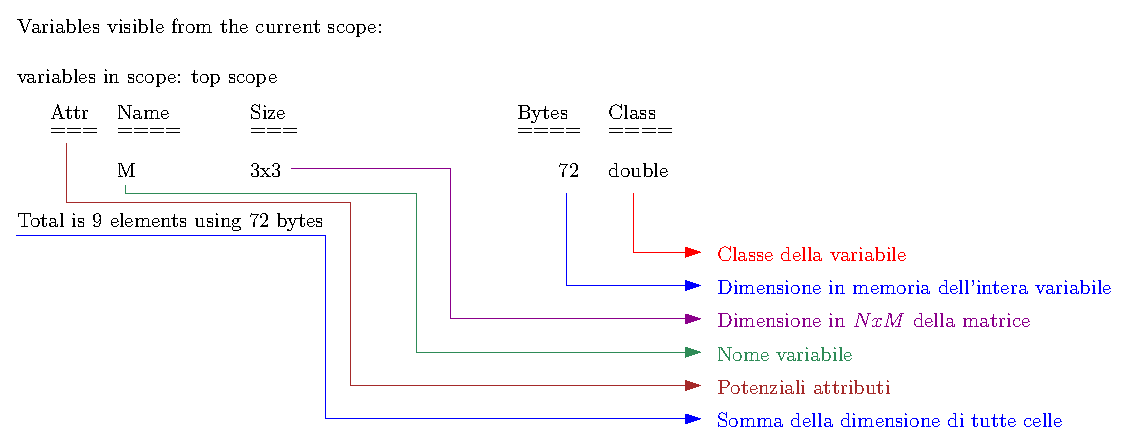
\includegraphics[width=15cm]{img/finiti/whos.eps}
  \caption{descrizione dell'interfaccia di funzione}
  \label{fig:interffun}
\end{figure}
\begin{notab}
  Anche la variabile singola viene vista come una matrice 1x1, da questo si
  denota che come il suo cugino Matlab è un software pensato per elaborare
  prodotti matriciali, infatti, il nome Matlab non sta per \texttt{Mathematic
    lab} ma per \texttt{Matrix Lab}. 
\end{notab}
\subsection{Tipi variabile}
\label{sec:tipivariabile}

\begin{table}[ht]
  \centering
  \begin{tabular}{llll}
    {\bf Nome} & {\bf Descrizione} & {\bf Dimensione} & {\bf Cifre rappresentabili}\\\hline
    \lstinline|double| ({\bf default}) & double-precision array & 8byte & $\pm1.79769x10^{308}$ a $\pm2.22507x10^{-308}$\\\hline
    \lstinline|single| & single-precision array & 4byte & $-2.1475x10^9$ a $2.1475x10^9$\\\hline 
    \lstinline|int8| & Array di interi con segno & 8bit & $-128$ a $127$\\\hline
    \lstinline|int16| & Array di interi con segno & 16bit & $-32768$ a $32767$ \\\hline
    \lstinline|int32| & Array di interi con segno & 32bit & $-2.1475x10^9$ a $2.1475x10^9$\\\hline 
    \lstinline|int64| & Array di interi con segno & 64bit & $-9.2234x10^{18}$ a $9.2234x10^{18}$\\\hline
    \lstinline|uint8| & Array di interi senza segno & 8bit & $255$\\\hline
    \lstinline|uint16| & Array di interi senza segno & 16bit & $65535$ \\\hline
    \lstinline|uint32| & Array di interi senza segno & 32bit & $4.2950x10^9$\\\hline 
    \lstinline|uint64| & Array di interi senza segno & 64bit & $1.8447x10^{19}$\\\hline
  \end{tabular}
  \caption{Tipi variabile}
  \label{tab:tipivariabile}
\end{table}
\begin{oss}
  Questa rapresentazione in memoria vale per la singola cella, quindi bisogna
  moltiplicare il paso per il numero di celle dello stesso tipo. Il programma
  peserà quanto il numero complessivo delle variabili presenti.
\end{oss}

\paragraph{Le stringhe --}
Un altro tipo di variabile però implicita sono le stringhe che il programma può
gestire, nel sequente modo \lstinline|str = "string x"| e la stampa di stringa
viene fatta con un semplice \lstinline|printf(str)|.
\clearpage
\subsubsection{Cosa stampa e cosa no}
Nel linguaggio di Matlab e Octave vengono stampate tutte le associazioni,
funzioni e inizializzazioni che non terminano con il ``{\color{red};}''.

\subsection{Impostazioni e formati}
\label{sec:formImp}
\begin{table}[ht]
  \centering
  \begin{tabular}{lll}
    {\bf Nome} & {\bf Descrizione} & {\bf Visuale}\\\hline
    \lstinline|rat| & Aspetto rateo (invece dei numeri reali rende numeri frazionari) & 1/2\\\hline
    \lstinline|short| & Formato breve a decimale fisso con 4 cifre dopo la virgola. (\textit{default}) & 0.5000\\\hline
    \lstinline|long| & Formato lungo a decimale fisso con 15 cifre dopo la virgola per & 0.500000000000000\\
                     &  i valori doppi e 7 cifre dopo la virgola per i valori singoli. \\\hline
    \lstinline|shortE| & Formato breve in annotazione scientiica con 4 cifre dopo la virgola & 5.0000e-01\\\hline
    \lstinline|longE| & Formato lungo a decimale fisso con 15 cifre dopo la virgola per & 5.000000000000000e-01\\
               & i valori doppi e 7 cifre dopo la virgola per i valori singoli.\\\hline
    \lstinline|shortG| & Formato breve, decimale fisso o notazione scientifica, a seconda & 0.5000\\
               & di quale sia più compatto, con un totale di 5 cifre.\\\hline
    \lstinline|longG| & Formato lungo a decimali fissi o notazione scientifica, qualunque & 0.500000000000000\\
               & sia il più compatto, con un totale di 15 cifre per i valori doppi e\\ & 7 cifre per i valori singoli.\\\hline
    \lstinline|shortEng| & Breve notazione ingegneristica (l'esponente è un
                           multiplo & 500.0000e-003\\
    
               &di 3) con 4 cifre dopo la virgola.\\\hline
    \lstinline|longEng| & Notazione ingegneristica lunga (l'esponente è un multiplo di 3) & 500.000000000000000e-003\\ & con 15 cifre significative.\\\hline
    \lstinline|+|&Formato positivo/negativo con caratteri +, - e vuoti visualizzati & +\\
               & per elementi positivi, negativi e zero.\\\hline
    bank & Formato valuta con 2 cifre dopo la virgola. & 0.50 \\\hline
    hex & Rappresentazione esadecimale di un numero binario & 3fe0000000000000 \\
               & a doppia precisione.\\\hline 
  \end{tabular}
  \caption{Impostazioni e formati}
  \label{tab:form}
\end{table}
\begin{notab}
  È possibile salvare il formato in una variabile con il comando \lstinline|fmt = format("nomeFormato")|
  per poi riutilizzarlo in seguito richiamando \lstinline|format(fmt)|. Altro aspetto esso può cambiare durante lo script quindi è possibile ripotare un dato
  in un formato di stampa e uno in un altro.
\end{notab}

\chapter{Derivate Parziali}
\section{Derivate parziali di primo grado}
\begin{defi}
  Sia $f(x,y)$ una funzione di due variabili definita in un punto interno ad $A$\\
  Consideriamo un interno circolare di $P(x_0,y_0),I(x_0,y_0), \delta$, in netto sulla retta $y=y_0$ e
  incrementa la $x_0$ passante da $x_0$ a $x_0+h$. Ho così un punto $P(x_0+h,y_0)\in A$.\\
  Definisco il rapporto di $f(x,y)$ nella sola $x$
  \begin{equation}
    \frac{f(x_0+h,y_0)-f(x_0,y_0)}{h}
  \end{equation}
  $f(x,y)$ si definisce {\color{red} derivabile parzialmente} se $\exists \lim\limits_{h\to 0}\frac{f(x_0+h,y_0)-f(x_0,y_0)}{h} = l\in R$ reale e finito.
  \begin{equation}
    \frac{\partial f}{\partial x} =fx=\lim\limits_{h\to 0}\frac{f(x_0+h,y_0)-f(x_0,y_0)}{h}
  \end{equation}
  Analogamente, considero un interno di $P(x_0,y_0), I(x_0,y_0),\delta$. Mi ruoto sulla retta $x=x_0$ e
  incremento la $y_0$ passando da $y_0$ a $y_0+k$. Ho così un punto $P(x_0,y_0+h)\in A$.\\
  Definisco il rapporto ingrementale di $f(x,y)$ nella sola $y$
  \begin{equation*}
    \frac{f(x_0+k,y_0)-f(x_0,y_0)}{k}
  \end{equation*}
  {\color{red} derivabile parzialmente} se $\exists \lim\limits_{h\to 0}\frac{f(x_0+h,y_0)-f(x_0,y_0)}{h} =
  l\in R$ reale e finito.\\
  Se in un punto ($x,y$) esistono entrambi le derivate parziale si dice che la funzione è {\color{red} derivabile}
  in (x,y) inoltre se $f$ è derivabile in ogni punto $(x,y)\in A$, si dice che f è derivabile in $A$.
\end{defi}
\subsection{Significato geometrico}
\begin{itemize}
\item Lo derivata prima par parziale in $P$ è $fx(x_0,y_0)$, è la tangente alla curva che si crea intersecando
  $f(x,y)$ con il piano $y=y_0$
\item La derivata prima parziale in $P$, $fy(x_0,y_0)$ è la tangente alla curva che si
  crea intersecando $f(x,y)$ con il piano $x=x_0$
\end{itemize}
Se esistono entrambe allora le due rette tangenti alle sezioni della funzione individuano il piano tangente al
solido nel punto $P(x_0,y_0,z)$
\section{Derivata parziale seconde}
\begin{defi}
  Sia $f(x,y)$ una derivabile e siano definite in un deminio le due derivate parziali
  \begin{equation*}
    \begin{matrix}
      f_x(x,y) & f_y(x,y)
    \end{matrix}
  \end{equation*}
  Tali funzioni passano a loro volta essere derivabili e si ottengono così le derivate seconde parziali di
  $f(x,y)$
  \begin{center}
    \Tree[.$f(x,y)$ [.$f_x(x,y)$ $f_{xx}(x,y)$ $f_{xy}(x,y)$ ] [.$f_y(x,y)$ $f_{yx}(x,y)$ $f_{yy}(x,y)$ ] ]
  \end{center} 
\end{defi}
\begin{multicols}{3}
  \begin{equation*}
    \begin{matrix}
      f_{yx}(x,y)\\
      \text{ derivata prima rispetto a}\\
      \text{ y poi rispetto a rispetto a x}
    \end{matrix}
  \end{equation*}
  \begin{equation*}
    \begin{matrix}
      f_{yx}(x,y)\\
      f_{yx}(x,y)
    \end{matrix}
    \text{ derivata seconde pure}
  \end{equation*}
  \begin{equation*}
    \begin{matrix}
      f_{yx}\\
      f_{yx}
    \end{matrix}
    \text{ derivata seconde resto}
  \end{equation*}
\end{multicols}
con $n$ variabili si hanno $n^2$ derivate seconde parziali -- Spesso le derivate seconde sono disposte in
una matrice quadrata, detta {\tt hessiana}, con il sinbolo $D^2$
\begin{equation}
  D^2f=\begin{bmatrix}
         f_{xx} & f_{xy}\\
         f_{yx} & f_{yy}
       \end{bmatrix}
       \text{n variabili} \to n*n
\end{equation}
Se esistono le quanto derivate di f, nel punto (x,y), si dice che $f$ è dirivabile due volte in $(x,y)$. Se
ciò accade $\forall (x,y)\in A$, $f$ è derivabile due volte nell'insieme A.
\subsection{Teorema di Schwarz (Dell'invertibilità dell'ordine di derivazione)}
\begin{teorema}
  Sia $f(x,y)$ definita in $D$ e derivabile due volte $\forall (x,y) \in D$.\\
  Se le derivate seconde in $(x_0,y_0)$ $f_{xy}(x_0,y_0)$ e $f_{yx}(x_0,y_0)$ sono continue in ($x_0,y_0$) allora\\
  risulta $f_{xy}(x_0,y_0)=f_{yx}(x_0,y_0)$.
\end{teorema}
In generale se vale il teorema di Schwarz, la matrice Hessiana può essere scritta come
\begin{equation*}
  H=D^2f=\begin{bmatrix}
           f_{xx} & f_{xy}\\
           f_{xy} & f_{yy}
         \end{bmatrix}
         = \begin{bmatrix}
             f_{xx} & f_{yx}\\
             f_{yx} & f_{yy}
           \end{bmatrix}
\end{equation*}
$det H= f_{xx}*f_{yy}-(f_{xy})^2=f_{xx}*f_{yy}-(f_{yx})^2$
\section{Massimi e minimi relativi}
\begin{defi}
  Sia $f(x,y)$ una funzione definita in un insieme D, un punto $p_0(x_0,y_0)\in D$, si dice di {\color{red}
    massimo relativo} per la funzione se esiste intorno circolare di $P_0$ per cui il valore assunto della
  funzione nei punti dell'interno è minore o uguale a quello assunto in $P_0$.\\
  Analogamente un punto $P_0(x_0,y_0)$ si dice di {\color{red} minimo relativo} per la funzione se esiste un
  interno circolare di $P_0$ per cui il valore assunto dalla funzione nei punti dell'intorno è maggiore o uguale.
  \begin{equation*}
    \begin{matrix}
      \exists I_{(x,y),\delta}:\forall (x,y)\in I_{(x,y),\delta} & f(x_0,y_0)\geq f(x,y) & \text{Massimo relativo}\\
      \exists I_{(x,y),\delta}:\forall (x,y)\in I_{(x,y),\delta} & f(x_0,y_0)\leq f(x,y) & \text{Minimo relativo}
    \end{matrix}
  \end{equation*} 
\end{defi}
\subsection{Teorema di Fermat}
\begin{teorema}
  Sia $f(x,y)$ derinita in D e derivabile in un punto $P_0 (x_0,y_0)$\\
  Se in $P_0(x_0,y_0)$ $f(x,y)$ ha un massimo o un minimo relativo, allora le derivate prime
  parziali si annullano ($\nabla f=0$ gradiente nullo). La pendenza della tangente è zaro un
  massimo o minimo.
\end{teorema}
\subsubsection{Gradiente}
Sia $f(x,y)$ una funzione derivabile in un punto (x,y), cioè esistano in (x,y) le due derivate
parziali $f_x$ e $f_y$.\\
Si definisce {\color{red} gradiente} di f(x,y) nel punto (x,y): i vettore $\nabla f$ le cui componenti sono le derivate parziali di f(x,y).
\begin{equation}
  \nabla f(x,y) \equiv (f_x(x,y); f_y(x,y))
\end{equation}
\subsubsection{Massimi e minimi -- condizione necessaria}
\begin{defi}
  Se $P_0(x_0,y_0)$ è un punto di massimo/minimo relativo il gradiente è nullo. Così di massimo
  o minimo relativo interni al dominio della funzione f vanno ricercati tra i punti che annullano
  la funzione f. Pertanto un punto critico per una funzione derivabile e un punto in cui si
  annulla il gradiente della funzione.
\end{defi}
\subsection{Differenziabilità}
\begin{defi}
  Sia $f(x,y)$ definita in D e $P_0(x_0,y_0)\in D$. In $P_0, z=f(x_0,y_0)$, incremento la $x_0$
  di un h e la $y_0$ di un k.\\
  Così passo da $P_0(x_0,y_0)$ a $P(x_0+h,y_0+k)$. La funzione avrà avuto un certo incremento
  \begin{equation*}
    f(x+h,y_0,y_0+k)-f(x_0,y_0)
  \end{equation*}
  Si definisce {\color{red}differenziale} in $P_0(x_0,y_0)$ se
  $\exists A,B \in R: f(x_0+h,y_0+k)-f(x_o,y_0)=Ah+Bk+o(\sqrt{h^2+k^2})$, cioè se esistono
  due costanti reali A e B per cui l'increm,ento di $f(x,y)$ che si ha passando da $P_0$ a $P$
  si può riscrivere come somma di una parte lineare $Ah+Bk$ e di un infinitesimo di ordine
  superiore a $\sqrt{h^2+k^2}$ (\underline{distanza di $P_0$ da $P$}).\\
  Se $f(x,y)$ ammette derivate prime parziali le due costanti A e B sono:
  \begin{equation*}
    \begin{cases}
      A=fx(x_0,y_0)\\
      B=fy(x_0,y_0)
    \end{cases}
  \end{equation*}
  e il differenziale diventa
  \begin{equation}
    f(x_0+h,y_0+k) - f(x_0,y_0)=fx(x_0,y_0)h+fy(x_0,y_0)k+o(\sqrt{h^2+k^2})
  \end{equation}
\end{defi}
\begin{esempio}
  verificare che $z=xy$ è differenziale $\forall (x_0;y_0)\in R^2$, se z è differenziale\\
  $\to f(x_0+h,y_0+k) - f(x_0,y_0)=fx(x_0,y_0)h+fy(x_0,y_0)k+o(\sqrt{h^2+k^2})$ dove
  \begin{equation*}
    \begin{cases}
      A=fx(x_0,y_0)\\
      B=fy(x_0,y_0)
    \end{cases}
  \end{equation*}
  se z è derivabile in ($x_0,y_0$).
  \begin{equation*}
    f(x_0+h,y_0+k) =\underbrace{(x_0+h)(y_0+k)}_{\text{\shortstack{Sostituisco}}}=x_0y_0+x_0k+y_0h+hk
  \end{equation*}
  \begin{multicols}{3}
    $f_x=y\text{ }fx(x_0,y_0)=y_0$\\
    $f$ è derivabile in $(x_0,y_0)$\\
    $f_y=x$\\
    $A=y_0$\\
    $f_y(x_0,y_0)=x_0$\\
    $D=x_0$
  \end{multicols}
  \begin{equation*}
    \begin{matrix}
      f(x_0+h,y_0+k) - f(x_0,y_0)=Ah+Bk+o(\sqrt{h^2+k^2})\\
      \not{x_0y_0}+\not{x_0k}+hk-\not{x_0y_0}=\not{y_0h}+\not{x_0k}+o(\sqrt{h^2+k^2})\\
      hk=o(\sqrt{h^2+k^2})
    \end{matrix}
  \end{equation*}
  detto quindi dimostrare che $\lim\limits_{h\to 0 k\to 0}\frac{hk}{\sqrt{h^2+k^2}}=0$
  e poi passo alle coordinate polari:
  \begin{equation*}
    \begin{matrix}
      h=\rho \cos \theta\\
      k=\rho \sin \theta & \lim\limits_{\rho\to 0} \frac{\not{e} \cos\theta* \not{e} sin\theta}{\not{e}^2}& z=xy \text{ defferenziale } \forall (x_0,y_0)\in R^2\\
      e^2=h^2+k^2\\
      h\to0,k\to 0,\rho \to 0\\
    \end{matrix}
  \end{equation*}  
\end{esempio}
\subsection{Tutte le funzioni differenziali sono continue}
Sia $f(x,y)$ differenziabile $(x_0,y_0)$, allora $f(x,y)$ è continua in $(x_0,y_0)$
\begin{multicols}{2}
  \paragraph{Ip:}
  \begin{equation*}
    f(x,y) \text{ differenziabile in } (x_0,y_0)
  \end{equation*}
  \paragraph{Th:}
  \begin{equation*}
    f(x,y) \text{ è continua in } (x_0,y_0)
  \end{equation*}
\end{multicols}
\begin{proof}
  Poiché $f(x,y)$ è differenziabile in ($x_0,y_0$) vale la relazione
  \begin{equation*}
    f(x_0+h,y_0+k) - f(x_0,y_0)=Ah+Bk+o(\sqrt{h^2+k^2})
  \end{equation*}
  Se $f(x_0,y_0)$ è continua in $(x_0,y_0)$
  \begin{equation*}
    \lim_{h\to 0\text{ } k\to 0}f(x_0+h,y_0+k) - f(x_0,y_0)=0
  \end{equation*}
  Calcolo il limite a destra per $h\to 0$ $k\to 0$
  \begin{equation*}
    \lim_{h\to 0\text{ } k\to 0}\underbrace{Ah}_0+\underbrace{Bk}_0+o\underbrace{(\sqrt{h^2+k^2})}_0=0 \text{ per cui $f(x,y)$ è continua in ($x_o,y_0$)}
  \end{equation*} 
\end{proof}
\subsection{Tutte le funzioni differenziali sono derivabili}
Sia $f(x,y)$ differenziabile in un punto ($x_0,y_0$). Allora $f(x,y)$ è derivabile in
$(x_0,y_0)$
\begin{multicols}{2}
  \paragraph{Ip:}
  \begin{equation*}
    f(x,y) \text{ differenziabile in } (x_0,y_0)
  \end{equation*}
  \paragraph{Th:}
  \begin{equation*}
    f(x,y) \text{ è derivabile in } (x_0,y_0)
  \end{equation*}
\end{multicols}
\begin{proof}
  Poiché $f(x,y)$ è differenziabile in ($x_0,y_0$) vale la relazione
  \begin{equation*}
    f(x_0+h,y_0+k) - f(x_0,y_0)=Ah+Bk+o(\sqrt{h^2+k^2})
  \end{equation*}
  divido entrambi per h e calcolo il limite per $h\to 0$
  \begin{equation*}
    \lim\limits_{h \to 0}\underbrace{\frac{f(x_0+h,y_0) - f(x_0,y_0)}{h}}_{\frac{\partial f}{\partial x}(x_0,y_0)=fx}=\underbrace{\frac{Ah+o(\sqrt{h^2})}{h}}_A
  \end{equation*}
  $fx(x_0,y_0)=A$\\
  Analogamente si demostra che $f_y(x_0,y_0)=B$. Qundi dato che esistono $f_x$ e $f_y$ in ($x_0,y_0$), $f(x,y)$ è derivabile in $(x_0,y_0)$ e in oltre $A=fx(x_0,y_0)$, $B=fy(x_0,y_0)$
\end{proof}

\printindex    
\end{document}